\documentclass{article}
\usepackage[english]{babel}
\usepackage[a4paper,top=2cm,bottom=2cm,left=3cm,right=3cm,marginparwidth=1.75cm]{geometry}

\usepackage{graphicx}
\usepackage{subcaption}
\usepackage[colorlinks=true, allcolors=blue]{hyperref}

\setlength\parindent{0pt}

\title{DRMBM (1994) remake}
\author{Christopher Ashford}
\date{September 2022}

\begin{document}
\maketitle

\tableofcontents

\section{Analysis}

\subsection{Introduction and Background}

Dr Robotnik’s Mean Bean Machine is a 1994 Westernised port of Puyo Puyo for the Sega Genesis/Mega Drive. It is a game that I have enjoyed throughout my childhood on many different forms – cheap emulation consoles, the Sega Mega Drive Collection for Xbox 360, using Fusion emulator on PC among other forms. However, all of these present glaring issues that directly affect the enjoyment of the player – emulation consoles usually are slow with clunky controllers and are not good for much else and thus are not practical to use permanently; the Sega Mega Drive collection on Xbox 360 suffers with a noticeable input lag problem, with inputs sometimes taking hundreds of milliseconds to be processed, directly affecting how fast you can play; PC emulation either results in a small or blurry image and makes it difficult to play with others or share your scores and achievements.

The goal of this project is to solve these problems by creating a superior, native PC remake of the game. Everything in the original game shall work exactly as in the original, including re-constructing the algorithms used for the playstyles of the various AI opponents. I also intend to include many quality of life improvements to solve the problems listed about: multiple customisable input method and handling will be supported, many algorithmic optimisations shall be made to improve performance, graphics shall be upscaled in a way that remains a crisp pixel look instead of introducing blur, an SQL web server will allow score and time leaderboards to exist and a replay file system shall be introduced to allow players to easily share gameplay. This project exists to create a superior version of DRMBM for a new generation to enjoy, as well as offering a way for modern Puyo Puyo players to enjoy the OPP rule set on modern devices.

If the goals above are reached, further extension goals include the introduction of my own custom AI opponents with algorithms designed for optimal, “perfect” gameplay and the use of web sockets to facilitate real-time online matches between two remote players.

\subsection{Alternative Solutions}

In this section I shall present my research on other Puyo Puyo games, compare the advantages and disadvantages of different versions from the perspective of the end user and take inspiration for my own project.

\subsubsection{Emulation}

\begin{figure}[h]
\centering
\begin{subfigure}{0.49\textwidth}
\centering
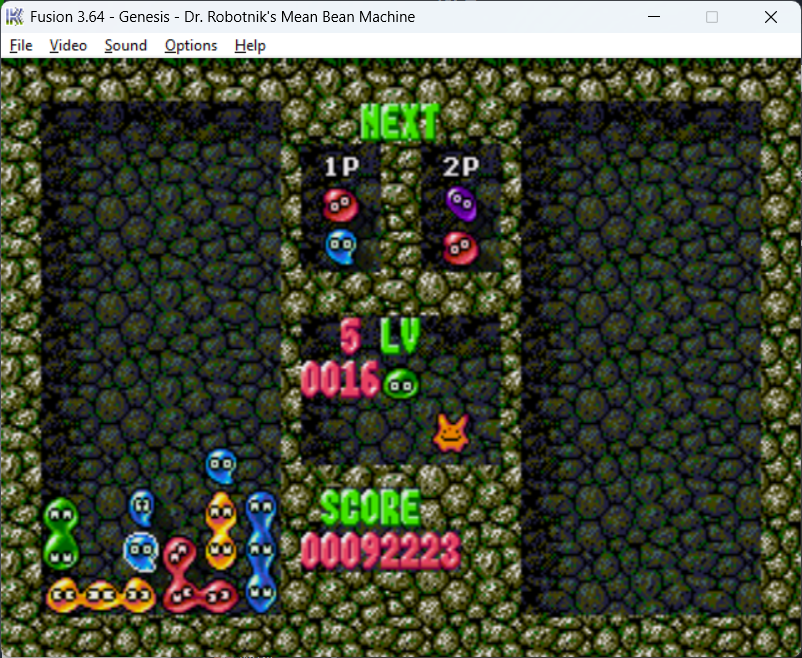
\includegraphics[width = \textwidth]{emulator1.png}
\caption{Fusion emulator}
\label{fig:emu1}
\end{subfigure}
\begin{subfigure}{0.45\textwidth}
\centering
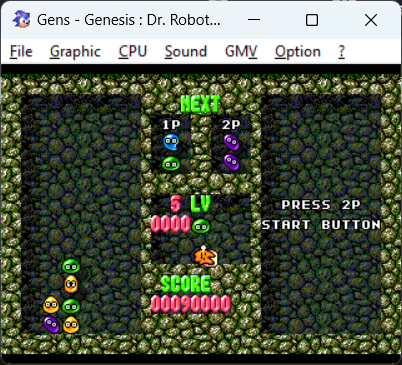
\includegraphics[width = \textwidth]{emulator2.png}
\caption{Gens emulator}
\label{fig:emu2}
\end{subfigure}
\caption{Some examples of emulators running the game}
\label{fig:combined}
\end{figure}

Link: cannot be provided due to specialised hardware being required to dump the ROM. Yet another disadvantage.

Many different emulators exist for the Sega Mega Drive, such as Fusion or Gens shown above, or the official Sega emulator that can be found on Steam. These are programs that accept a binary ROM dump of the original cartridge and attempt to emulate the code.
\vspace{0.3cm}

Advantages:

\begin{itemize}
    \renewcommand\labelitemi{--}
    \item Convenient for mass production and distribution.
    Sega can create one Mega Drive emulator and release an entire of library of games that use the same program
    \item True to the original experience.
    Since you are playing a copy of the original game, you can be sure you are getting an authentic experience
    \item While clunky, save states allow you to save high scores and progress through the story, as well as letting you manipulate sequences of beans
\end{itemize}

Disadvantages: 

\begin{itemize}
    \renewcommand\labelitemi{--}
    \item Resolution is locked at the console’s original and upscaling is blurry and unappealing
    \item Very static and not customisable. It is incredibly difficult to edit a ROM if you wanted to play with, for example, different handling or textures
    \item Saving progress is difficult
    \item Emulators are difficult to run and can easily lag on lighter hardware, running the game at higher levels can struggle on older processors
    \item It is impossible to play with friends remotely (or if it is possible, then it’s too difficult for the average user to achieve)
\end{itemize}

\subsubsection{B Puyo}

\begin{figure}[h]
\centering
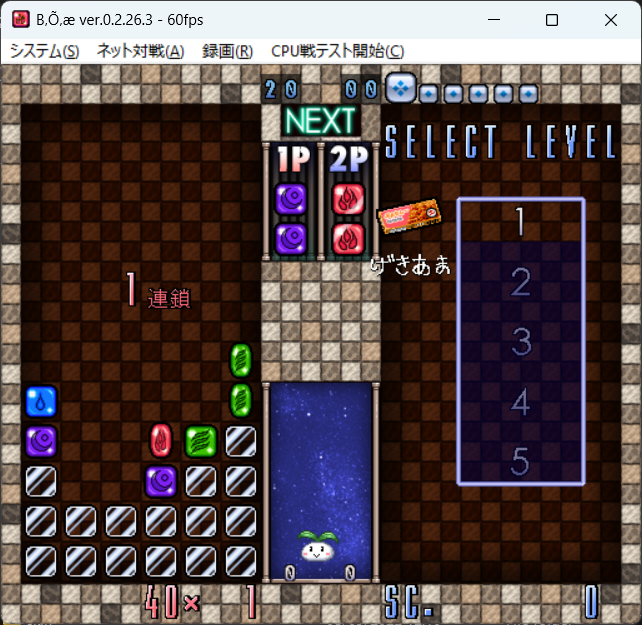
\includegraphics[width=0.3\textwidth]{bpuyo.png}
\caption{\label{fig:bpuyo}A screenshot of B Puyo. Some text is broken running on an English computer.}
\end{figure}
\begin{figure}[h]
\centering
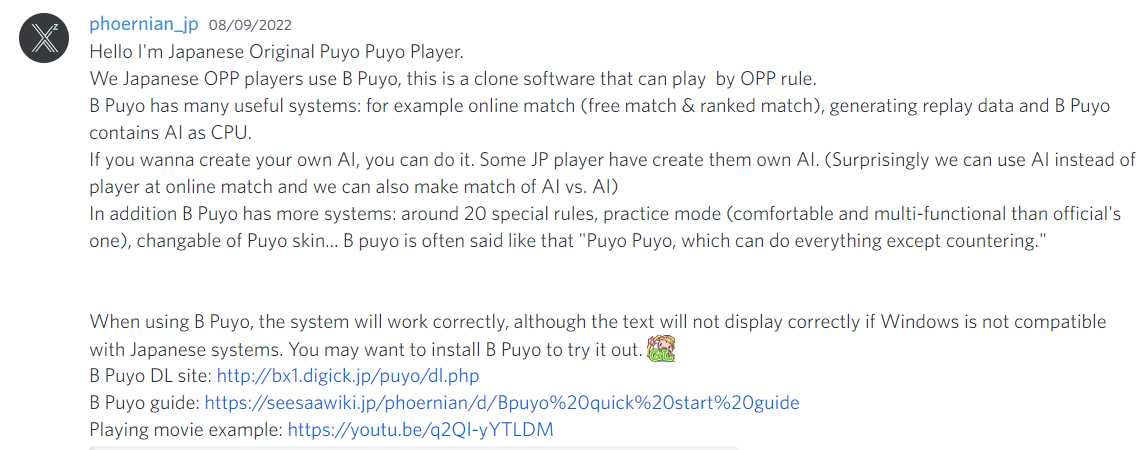
\includegraphics[width=1\textwidth]{discord.png}
\caption{\label{fig:discord}Information about B Puyo from a well known Japanese player.}
\end{figure}
Link: \href{http://bx1.digick.jp/puyo/dl.php}{http://bx1.digick.jp/puyo/dl.php}

B puyo is a popular online Puyo-clone recommended to me by the Japanese community.
\vspace{0.3cm}

Advantages:

\begin{itemize}
    \renewcommand\labelitemi{--}
    \item Custom textures, custom AI, custom rules, custom anything really
    \item Easy to use online multiplayer
    \item Great performance as a native PC program

\end{itemize}

\vspace{3cm}

Disadvantages: 

\begin{itemize}
    \renewcommand\labelitemi{--}
    \item Will only run on Windows, excluding Mac and Linux users
    \item The entire thing is in Japanese, with no translation options. Furthermore, servers are in Japan, creating ping issues for non-Japanese players. This is great for the Japanese community, but unfortunately disadvantages me as a Western player
    \item The resolution is locked to being a small window, making it uncomfortable to use on high-resolution displays
\end{itemize}

\subsubsection{Project GelaVolt}

\begin{figure}[h]
\centering
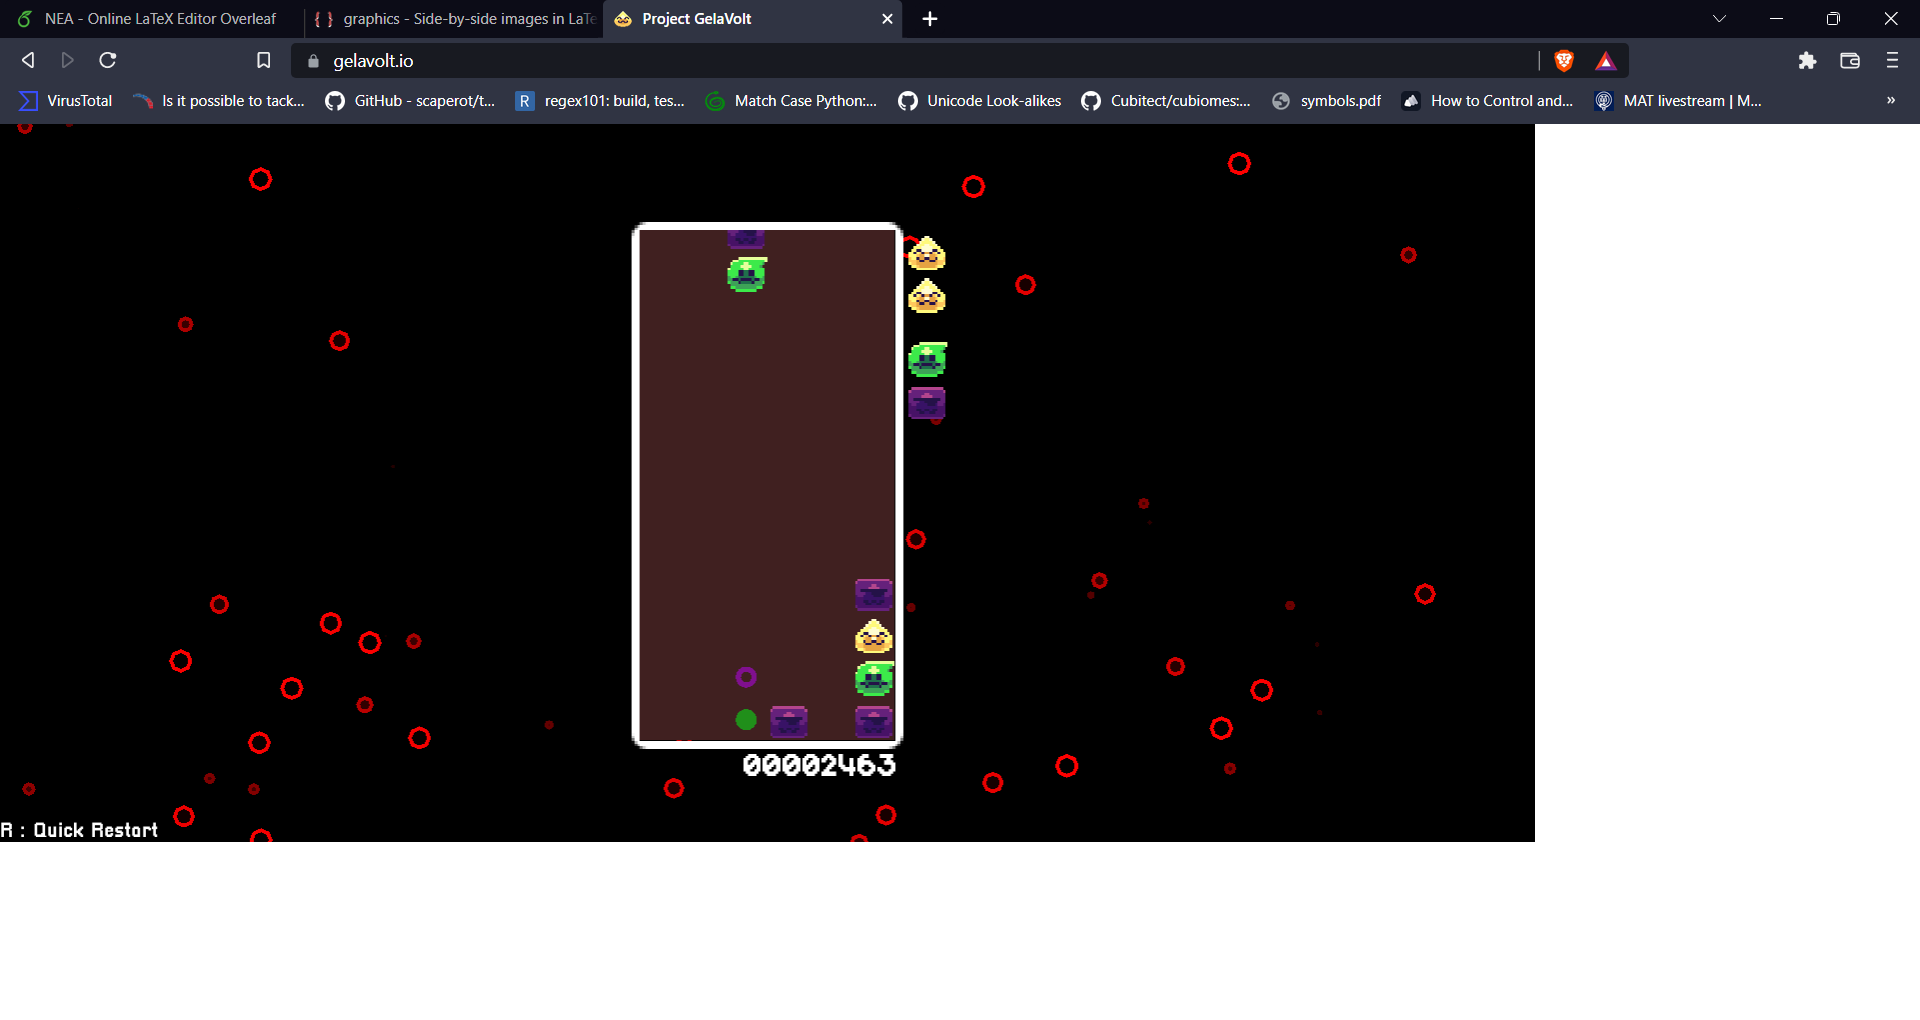
\includegraphics[width=1\textwidth]{gelavolt.png}
\caption{\label{fig:gelavolt}A screenshot of GelaVolt running in a chromium-based web browser.}
\end{figure}
Link: \href{https://gelavolt.io/}{https://gelavolt.io/}

To quote the game’s creator, “Project GelaVolt is a modern, techno-themed pixel art fangame of SEGA's Puyo Puyo series, one of Japan's most successful puzzle fighter franchises. Currently, GelaVolt is focused on the competitive aspects of the game and it's intended purpose is to help introduce people and help people get better at Puyo Puyo. However, if all goes well, GelaVolt will become a free alternative that plans to solve some of the communities problems: lack of players, lack of crossplay and lack of general quality netcode.” It is a Puyo-clone written in Haxe that runs in browsers.
\vspace{0.3cm}

Advantages:

\begin{itemize}
    \renewcommand\labelitemi{--}
    \item Appealing design
    \item Is lightweight and capable of running well in browsers
    \item Supports many different control schemes out of the box (controller, keyboard, etc.)
    \item Only version I’ve played that has hard drop
\end{itemize}

\vspace{0.7cm}

Disadvantages: 

\begin{itemize}
    \renewcommand\labelitemi{--}
    \item Multiplayer is in the works but is currently not supported at the time of writing
    \item Things such as textures are not customisable
    \item Is unstable and crashes regularly
\end{itemize}

\subsubsection{Puyo Puyo Tetris 2}

\begin{figure}[h]
\centering
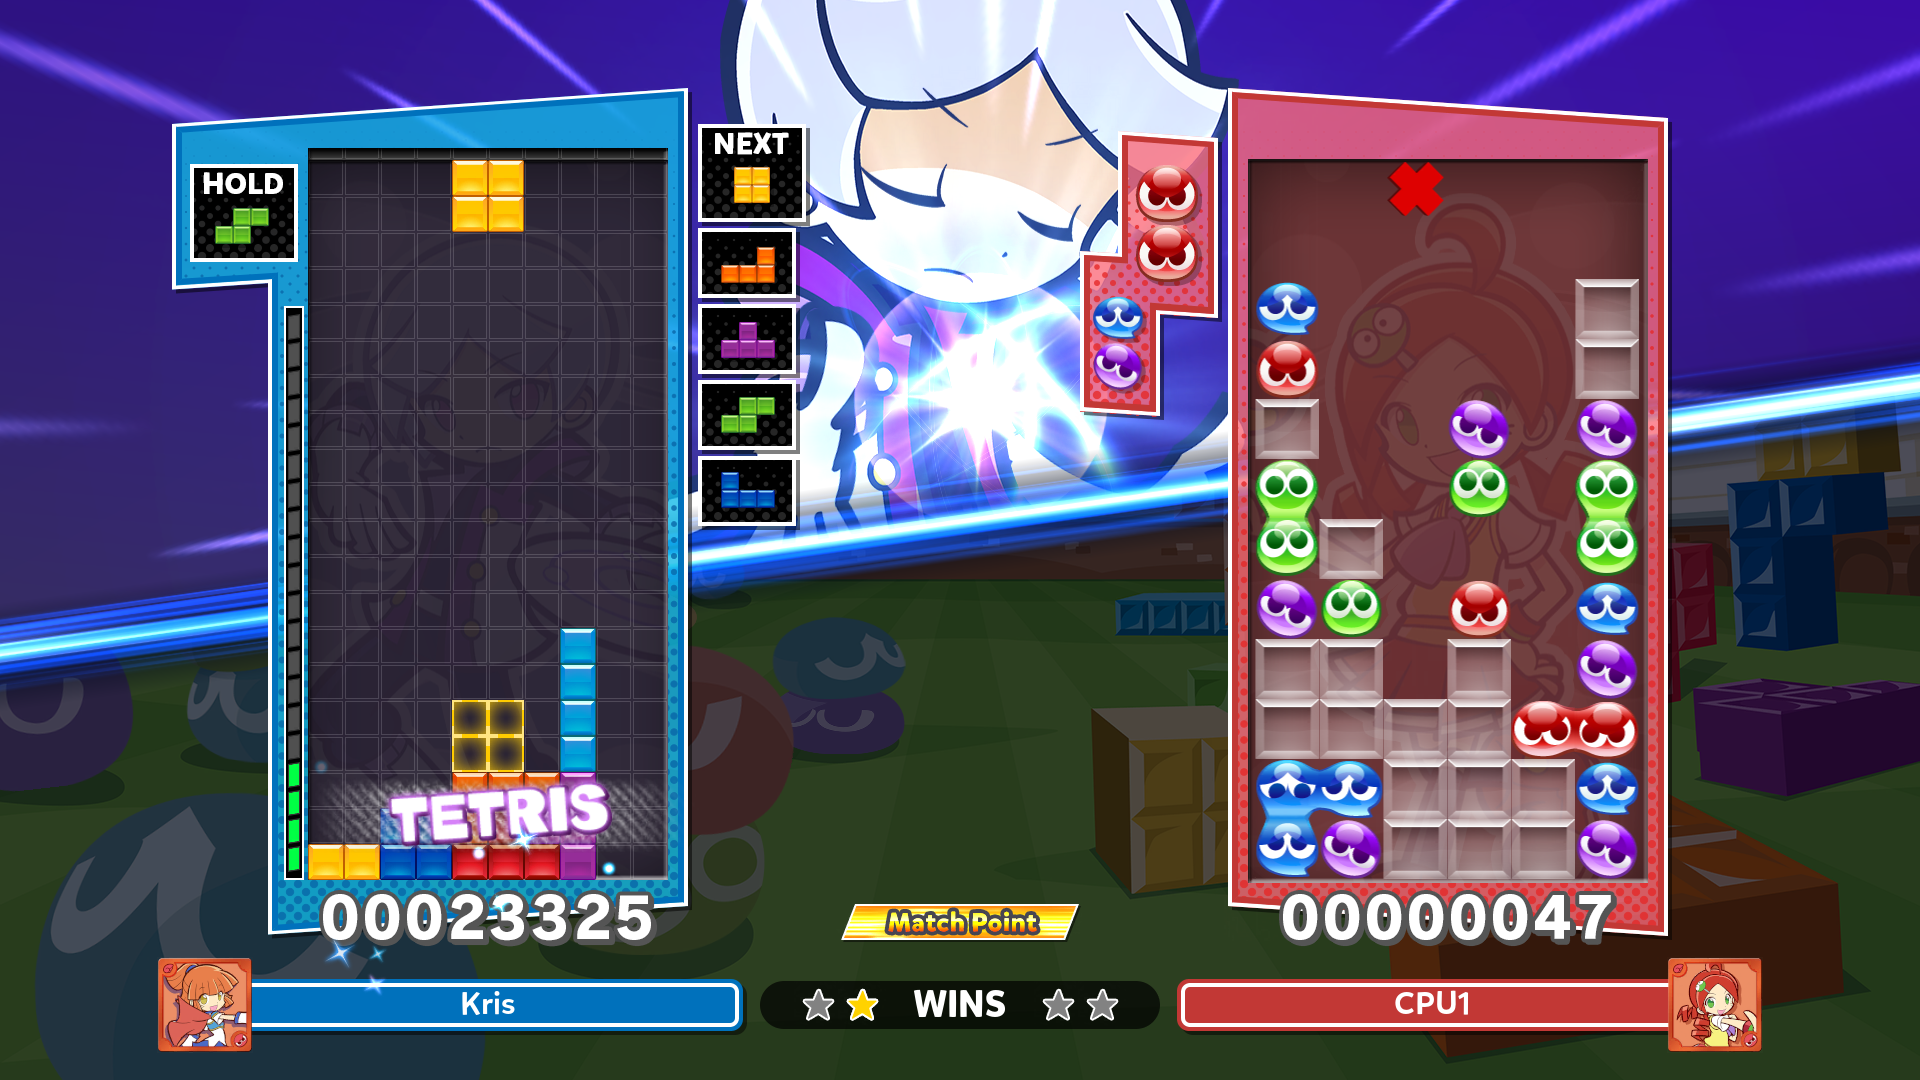
\includegraphics[width=1\textwidth]{ppt2.png}
\caption{\label{fig:ppt2}A screenshot of a versus battle, I'm playing Tetris and the CPU is playing Puyo Puyo.}
\end{figure}
Link: \href{https://store.steampowered.com/app/1259790/Puyo_Puyo_Tetris_2/}{https://store.steampowered.com/app/1259790/Puyo\_Puyo\_Tetris\_2/}

Puyo Puyo Tetris 2 is the latest Puyo Puyo game released by Sega and combines Puyo Puyo gameplay with Tetris, allowing players of both games to seamlessly play against one another. It has a full story and online mode.
\vspace{1cm}

Advantages:

\begin{itemize}
    \renewcommand\labelitemi{--}
    \item Cutesy art style is appealing to many, but can be swapped out with unlockable designs
    \item Being an official release, it is very stable with a consistent online multiplayer
    \item CPU opponents
    \item Fully voice-acted story with unique and creative characters
    \item Active modding community
\end{itemize}

Disadvantages: 

\begin{itemize}
    \renewcommand\labelitemi{--}
    \item Ranked multiplayer is fundamentally flawed as leaving matches is not punished
    \item CPU opponents fail to provide a challenge
    \item The game is very expensive, whereas all other options listed above are free
    \item Tsu ruleset, unable to be changed
\end{itemize}

\subsection{End User Input}

Being a popular game, many people enjoy the Puyo Puyo franchise, but the best people to survey for this project were the people who were most familiar with DRMBM specifically - speedrunners. A lot of the research in this document was greatly helped by the members of the "Puyo Speedrun" Discord server, and the contributers to the DRMBM-specific channel they have there.
In order to efficiently collect statistical end user input, a form was created using Microsoft Forms, a PDF version of which can be found here: \href{https://github.com/Kris-0605/nea/blob/master/documentation/NEA.pdf}{https://github.com/Kris-0605/nea/blob/master/documentation/NEA.pdf}

Question 1: Have you played Dr Robotnik's Mean Bean Machine before?
\begin{itemize}
    \renewcommand\labelitemi{--}
    \item Yes
    \item No
    \item Other Puyo Puyo game
\end{itemize}
Only one answer was permitted.

\begin{figure}[h]
    \centering
    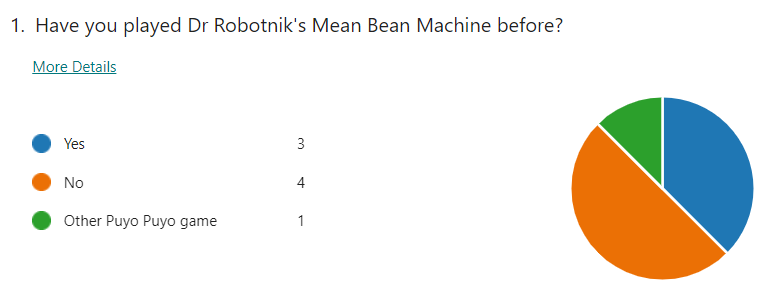
\includegraphics[width=0.8\textwidth]{survey1.png}
    \caption{\label{fig:survey1}Results to the first survey question.}
\end{figure}

The only notable thing about this question is that anyone who answered "No" was taken to the end of the form and was unable to answer any other questions. Thus, only 4 people continued to fill out the rest of the form.
\\\\
Question 2: Which modes in DRMBM are you experienced with and enjoy using?
\begin{itemize}
    \renewcommand\labelitemi{--}
    \item Scenario mode
    \item 1P VS. 2P mode
    \item Exercise mode
    \item Other
\end{itemize}
Any number of answers were pemitted.

\begin{figure}[h]
    \centering
    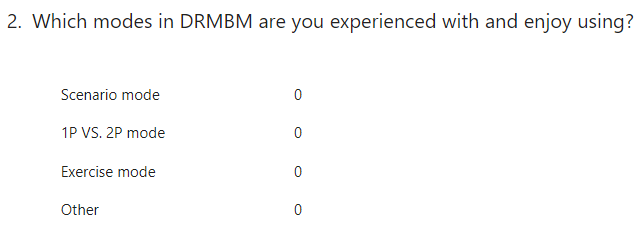
\includegraphics[width=0.8\textwidth]{survey2.png}
    \caption{\label{fig:survey2}Results to the second survey question.}
\end{figure}

No-one answered this question, thus nothing meaningful is gained from it.
\\\\
Structure
"This project is intended to both remake the original game in it's purest form, apply enhancements to it, thus the game will be split into two modes, that will from now on be referred to as "Classic mode" and "Enhanced mode". Classic mode is intended to be an exact recreation of the original game, and Enhanced mode should contain any additions and improvements."
\\\\
A message explaining some of the games structure that is important to understand when considering survey questions, which will be discussed further in the documented design section.
\\\\
Question 3: Consider scenario mode's password feature. Enhanced mode will allow the player to use save files that store additional data such as score, times and replays. What do you believe is the best way for the password menu to be implemented?
\begin{itemize}
    \renewcommand\labelitemi{--}
    \item Classic mode will use the same passwords from the original game in their original form, taking you to a level but not restoring data such as score
    \item Classic mode will generate new unique password that stores a hidden save file, so that the user is still required to use a password, but this password restores data such as score when used
    \item The password menu should be entirely replaced by save files in both modes
    \item Other
\end{itemize}
Only one answer was permitted.

\begin{figure}[h]
    \centering
    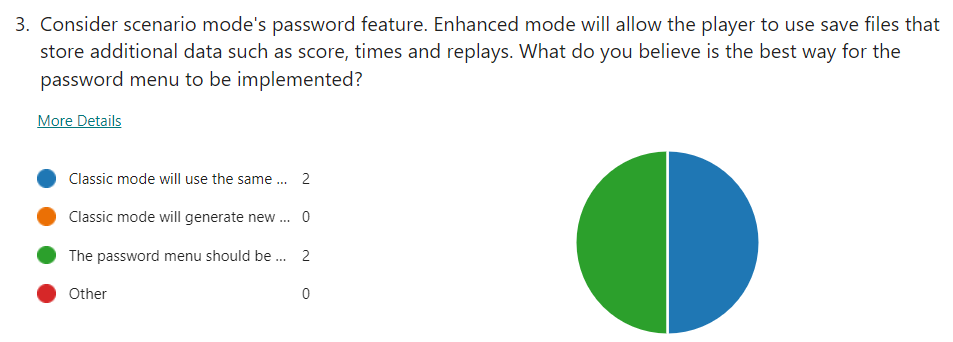
\includegraphics[width=0.8\textwidth]{survey3.png}
    \caption{\label{fig:survey3}Results to the third survey question.}
\end{figure}

The results to this question were an exact 50/50 split, thus I shall stick to my original plan of having Classic mode use passwords in their original form without any additional data, and using save files for enhanced mode.
\\\\
Question 4: What is your opinion on scenario mode's difficulty?
\begin{itemize}
    \renewcommand\labelitemi{--}
    \item Harder modes should be added to challenge more difficult players
    \item Easier modes should be added to help new players
    \item The difficulty options should remain the same in scenario mode, more customisable opponents should be available in a separate "training mode" in enhanced mode
    \item I don't believe any changes should be made
    \item Other
\end{itemize}
Any number of answers were pemitted.

\begin{figure}[h]
    \centering
    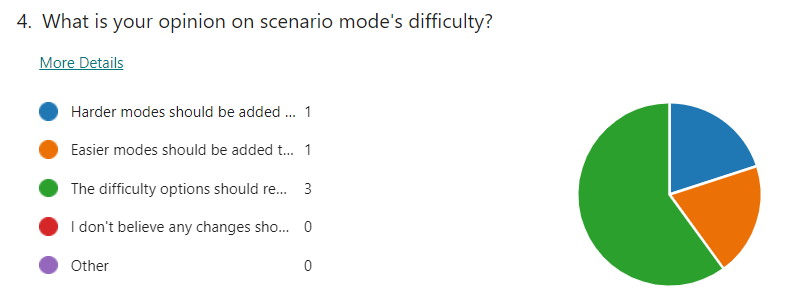
\includegraphics[width=0.8\textwidth]{survey4.png}
    \caption{\label{fig:survey4}Results to the fourth survey question.}
\end{figure}

The majority vote represented the solution that I believe would fit best and already planned on implementing: in both classic and enhanced mode, difficulty shall remain the same as in the original. However, in enhanced mode, you can play against customisable opponents, such as the same algorithms from scenario mode with different speeds, as well as new AI altogether.
\\\\
Question 5: The original game uses the OPP ruleset for scenario mode, the main difference being that garbage cannot be cancelled. What do you believe is the best configuration of rulesets?
\begin{itemize}
    \renewcommand\labelitemi{--}
    \item Classic mode scenario mode should use the OPP ruleset to recreate the original game and Enhanced mode should allow the user to choose before starting a save file
    \item Force OPP for scenario mode in both modes and allow players to choose Tsu when creating custom games
    \item Other
\end{itemize}
Only one answer was permitted.

\begin{figure}[h]
    \centering
    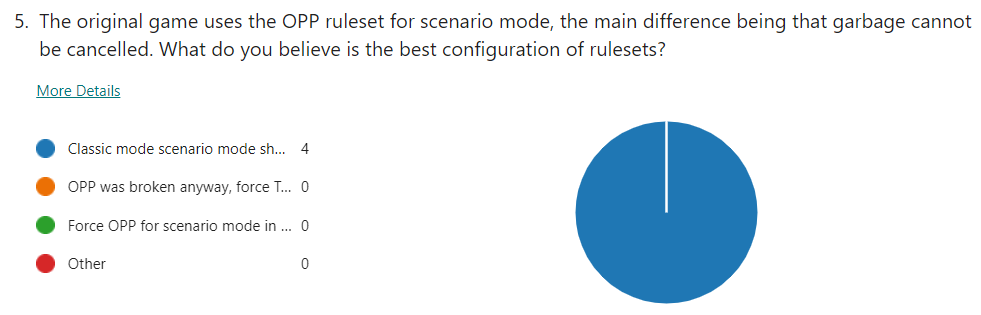
\includegraphics[width=0.8\textwidth]{survey5.png}
    \caption{\label{fig:survey5}Results to the fifth survey question.}
\end{figure}

The only unanimous result in the entire survey, as well as the solution I was planning on implementing. I will talk more about rulesets in the documented design section.
\\\\
Question 6: Do you have any other additions or comments regarding scenario mode?
This question permitted a text answer.

\begin{figure}[h]
    \centering
    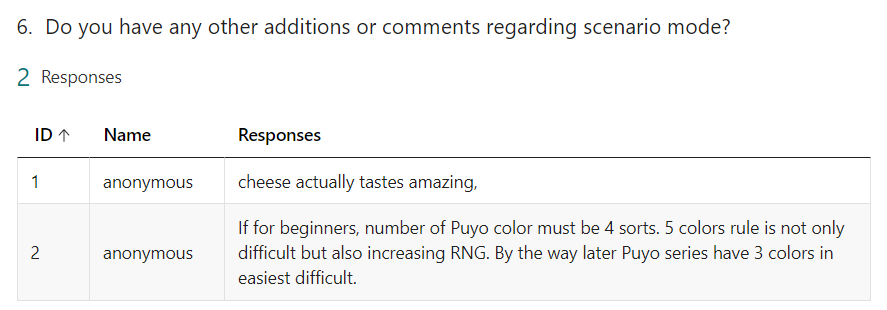
\includegraphics[width=0.8\textwidth]{survey6.png}
    \caption{\label{fig:survey6}Results to the sixth survey question.}
\end{figure}

Response ID 2 makes a very valid point. In newer versions of puyo puyo, difficulty settings change the number of colours that appear in play between 3, 4 and 5, whereas being an older game DRMBM uses 5 puyo colours in all difficulty modes. I will be sure to include the suggestion in enhanced mode.
\\\\
Question 7: While ambitious, the plan is to eventually include online multiplayer in the game for enhanced mode. Which of the following modes would you be interested in using? 
\begin{itemize}
    \renewcommand\labelitemi{--}
    \item Customisable private rooms that you can invite other players to
    \item Customisable public rooms, given in a listing that anyone can join
    \item Ranked multiplayer, with a rating system
    \item A super lobby (i.e. 20+ players)
    \item Other
\end{itemize}
Any number of answers were pemitted.

\begin{figure}[h]
    \centering
    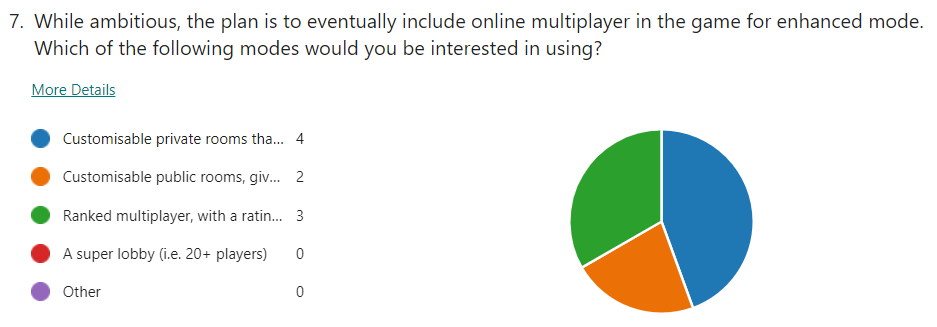
\includegraphics[width=0.8\textwidth]{survey7.png}
    \caption{\label{fig:survey7}Results to the seventh survey question.}
\end{figure}

All of the above are planned to be implemented, but the distribution of votes gives me a timeline with which to work on each feature.
\\\\
Question 8: When considering the Has Bean and Big Bean bonuses in exercise mode, which of the following statements do you agree with?
\begin{itemize}
    \renewcommand\labelitemi{--}
    \item Has Bean and Big Bean should be toggleable when playing exercise mode in enhanced mode
    \item Exercise mode attempts using Has Bean and Big Bean should use a separate leaderboard
    \item Has Bean and Big Bean should always be forced in exercise mode since they are part of the game mode, and should be toggleable when playing custom games
    \item Other
\end{itemize}
Any number of answers were pemitted.

\begin{figure}[h]
    \centering
    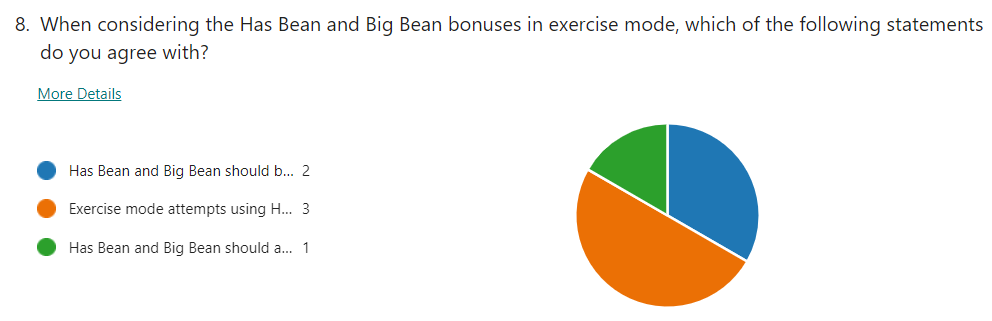
\includegraphics[width=0.8\textwidth]{survey8.png}
    \caption{\label{fig:survey8}Results to the eighth survey question.}
\end{figure}

The majority of people would like leaderboards to be split between runs that use Has Bean/Big Bean and runs that do not. This is surprising to me, but not particularly difficult to implement thus shall be included. This overrides the one person's comment about always forcing them.
\\\\
Question 9: In DRMBM, the score counter is capped at 99,999,999, and the puyo counter is capped at 9,999. In the original game, these counters froze on the event of a max out. How do you think a max out should be handled?
\begin{itemize}
    \renewcommand\labelitemi{--}
    \item In Classic mode, the counter should freeze, in Enhanced mode the counter should physically expand to accommodate more digits
    \item The counter should always freeze
    \item The counter should always expand
    \item Other
\end{itemize}
Only one answer was permitted.

\begin{figure}[h]
    \centering
    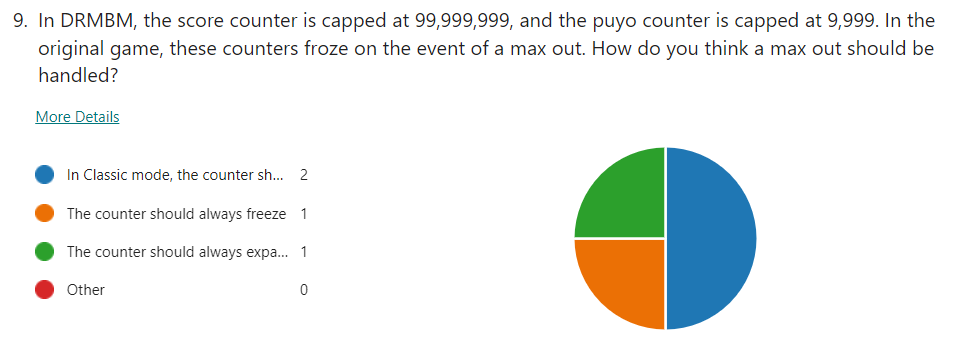
\includegraphics[width=0.8\textwidth]{survey9.png}
    \caption{\label{fig:survey9}Results to the ninth survey question.}
\end{figure}

A majority of people would like to implement the solution that I personally had in mind: freezing the counters in classic mode and allowing them to physically expand in enhanced mode, so this is what I shall implement. I understood that allowing the counters to freeze in classic mode would be important to keep because a popular speedrun of the game is trying to max out the score counter in the least possible time, and removing this bug would take away from one of the ways people enjoy the game.
\\\\
Question 10: As part of the project's requirements, I am going to include an online leaderboard. What stats do you think should be available as a leaderboard?
This question permitted a text answer.

\begin{figure}[h]
    \centering
    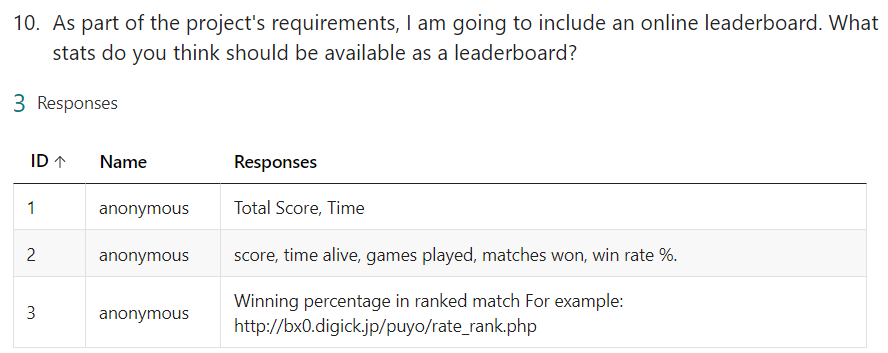
\includegraphics[width=0.8\textwidth]{survey10.png}
    \caption{\label{fig:survey10}Results to the tenth survey question.}
\end{figure}

These are all fairly generic examples, but I do appreciate the link provided to a Japanese ranked BPuyo leaderboard to use as an example.

\begin{figure}[h]
    \centering
    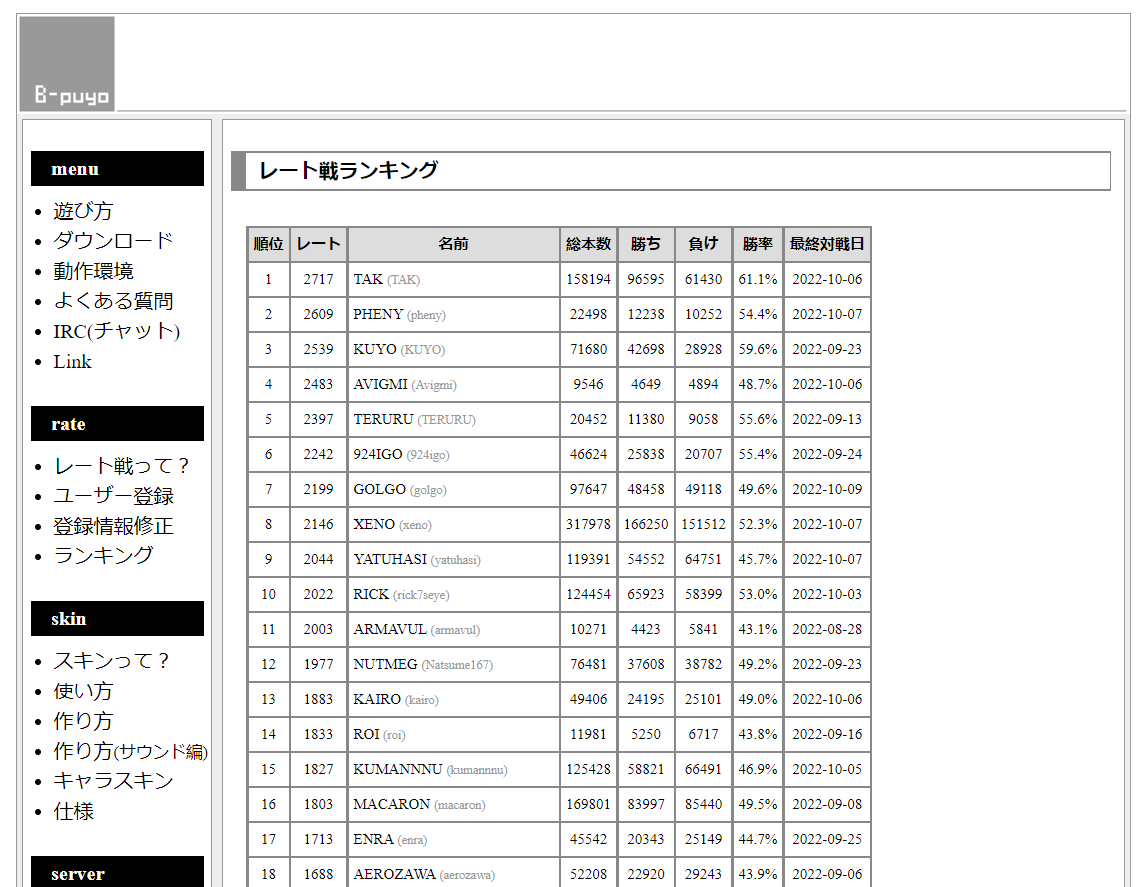
\includegraphics[width=0.8\textwidth]{bpuyo_leaderboard.png}
    \caption{\label{fig:bpuyo_leaderboard}The ranked leaderboard from the Bpuyo website.}
\end{figure}

Question 11: Enhanced mode will allow the game to support a 16:9 aspect ratio. What do you believe should be used to fill the space?
This question permitted a text answer.

\begin{figure}[h]
    \centering
    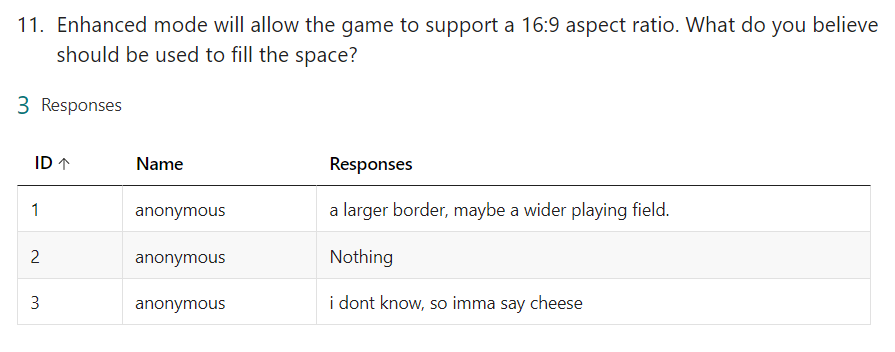
\includegraphics[width=0.8\textwidth]{survey11.png}
    \caption{\label{fig:survey11}Results to the eleventh survey question.}
\end{figure}

The solution to this problem remains to be determined, so I will probably fill it with empty space for now and see if I figure out something convenient later.
\\\\
Question 12: Below are other features that I plan to implement into Enhanced mode. Rate their importance.
The options contained within rows were:
\begin{itemize}
    \renewcommand\labelitemi{--}
    \item Custom texture support
    \item Custom handling settings
    \item Custom resolutions (any aspect ratio)
    \item Allow for custom AI and bots
    \item Simple modding API, mod installation built-in to the game
\end{itemize}
The options contained within columns were:
\begin{itemize}
    \renewcommand\labelitemi{--}
    \item I actively dislike this
    \item Would be nice to have, but not needed
    \item Should be included in final release
    \item Critical, prioritise this!
\end{itemize}

\begin{figure}[h]
    \centering
    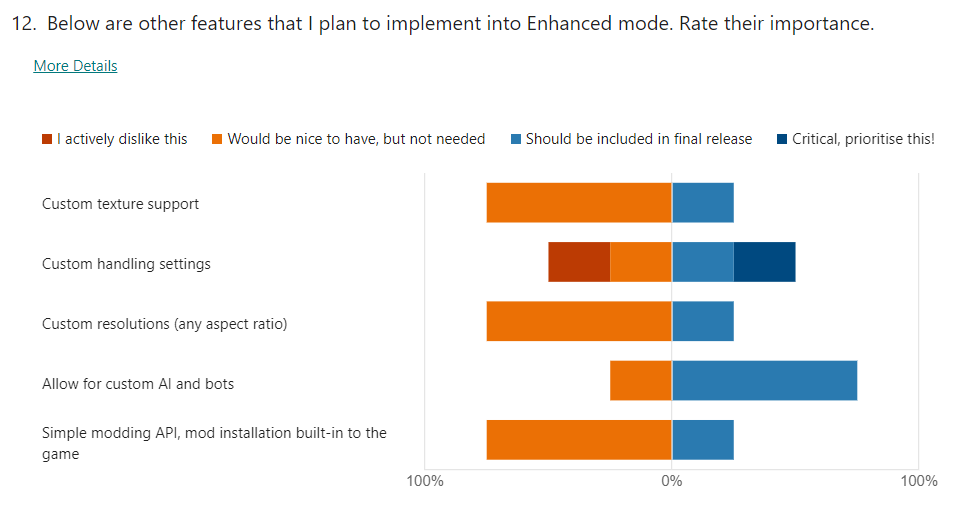
\includegraphics[width=0.8\textwidth]{survey12.png}
    \caption{\label{fig:survey12}Results to the twelth survey question.}
\end{figure}

All of the items listed are planned to be included, it is simply a matter of prioritising what the end user considers important.
For custom textures, 3 people said it would be nice to have and 1 said it should be in the final release. The inclusion of custom texture support itself is fairly trivial to implement due to the nature of having to import textures using the engine anyway, the time-consuming part would be writing documentation that explains how people can create their own texture packs that would be compatible with the game. I now know that this should not be prioritised.

Custom handling settings was the most devisive option, with each of the 4 applicants choosing separate options. I don't understand the rational behind actively disliking custom handling settings as the default will be the same as they are in the actual game, however it may be worth considering forcing certain handling settings in ranked matches or games that will be displayed on leaderboards; perhaps different leaderboards with enforced handling and custom handling? This will have to be considered.

Custom resolutions received the same reception as custom textures - it would be nice to have but isn't overly important. Different aspect ratios are actually especially challenging and non-trivial to implement. My original design for the engine involved scene data containing a background image variable, however this static image doesn't account for different resolutions and aspect ratios. Thus in order to account for future support for multiple aspect ratios, the engine must be coded to accept the background as a function that draws the background. Then when coding scenes, the specific scene can decide the solution that is most appropriate for drawing the background, whether that be a solid colour, stretching an image to fit a resolution, having multiple images to support multiple aspect ratios or some kind of tiling solution.

Custom AI and bots received a positive reception. I shall have to create an object that allows for the implementation of AI to create the CPUs in scenario mode, thus it shall be trivial to allow modders to run their own function within this class (with some kind of primitive virus protection by not allowing external modules to be accessed).

The described "modding API" will simply be an expanded version of what is described above - allowing users to modify their game by importing new objects written by other users that are compatible with the engine, at the user's own risk.

The survey was supposed to include a poll about replays, but unfortunately I forgot to include it. I can only assume it would be a desired feature.

\subsection{Input, Data Processing, Output}

The program is started with main.py. This script shall verify the integrity of local game assets using SHA hashing and querying a simple API on a web server, retrieving assets as necessary. Then, the script shall import Kris's Engine, an engine that shall be written and packaged by me with the game. 

Kris's Engine is built upon the idea of two fundamental class templates Scene and Entity, which shall be further described within the Documented Design section of this report. The engine shall first initalise itself, loading assets and creating the asynchronous networking thread. The engine shall then import the scene that is predefined by main.py, which will probably be title.py to load the title screen. From then, the engine shall use two threads: one for rendering and one for updating entities. Each entity must have the methods render and update, where the engine on seperate threads will call update 600 times per second and render a variable amount of time, that is able to be changed by the user, that will default to 60. The update method for an entity is responsible for data processing and the render method is responsible for any visual output that may be needed.

\begin{figure}[h]
\centering
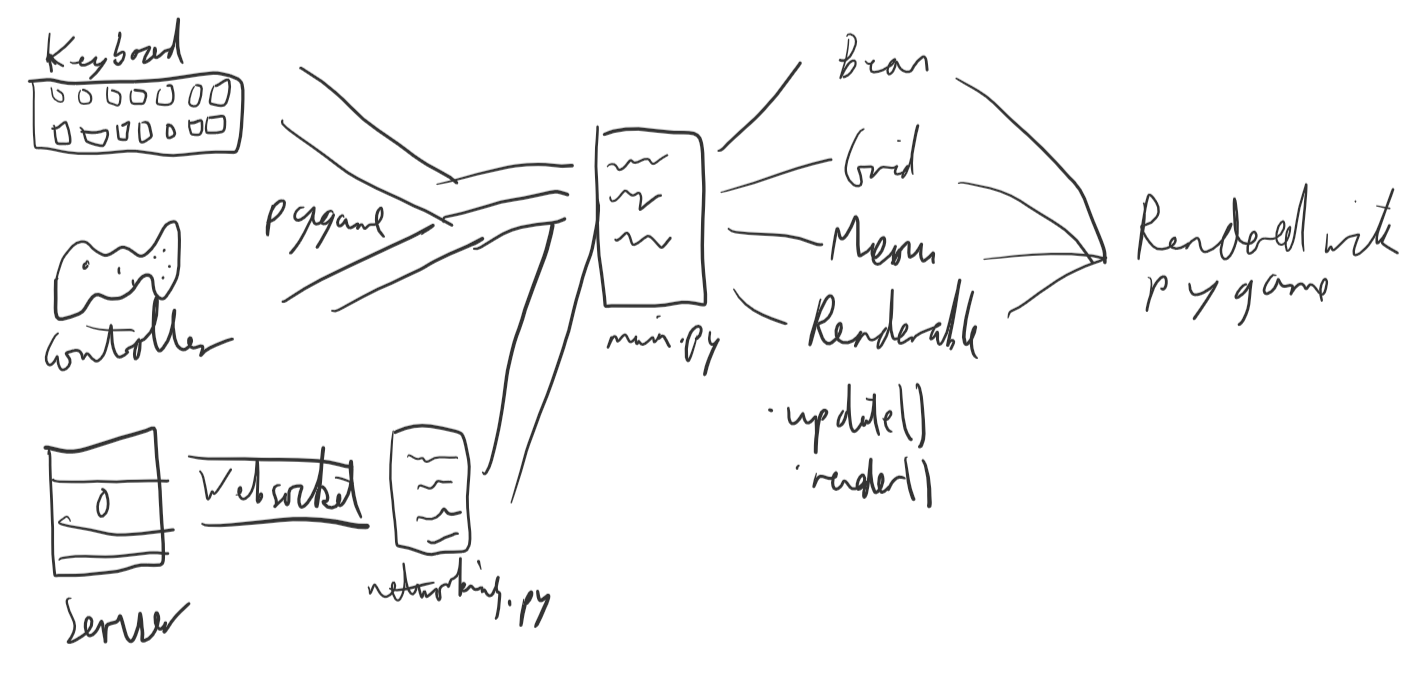
\includegraphics[width=1\textwidth]{idpo.png}
\caption{\label{fig:idpo}An Input, Data Processing, Output diagram.}
\end{figure}

\subsection{Goals}

\subsubsection{Main objectives}

\begin{itemize}
    \renewcommand\labelitemi{--}
    \item The project shall contain an engine module, which consists of an Engine class. This Engine class should:
    \begin{itemize}
        \renewcommand\labelitemi{--}
        \item Define the Scene and Entity classes, to be used as templates. These objects will be described further in depth in this document's Documented Design section.
        \begin{itemize}
            \item The Scene class should allow an object that inherits from it to:
            \begin{itemize}
                \item define what assets (images, sound files, etc) need to be present for a given scene.
                \item define some functions required for rendering a scene such as a function for rendering the background of a scene that works for different resolutions
                \item define what entities should be loaded in with a scene, their order and initialisation parameters
            \end{itemize} 
            \item Any object that inherits from the Entity class should:
            \begin{itemize}
                \item Define an update method which handles the data processing for a given entity.
                \item Define a render method which handles the output for a given entity, be that pygame rendering functions, console print statements, logging to a file, etc.
            \end{itemize}
        \end{itemize}
        \item Initialise pygame and take ownership of all pygame objects, such as the screen object being located at Engine.screen
        \item Initialise multiple threads:
            \begin{itemize}
                \item A thread shall be responsible for handling the update method of every entity that is owned by the Engine. The aim is to run this 600 times per second.
                \item A thread shall be responsible for handling the render method of every entity that is owned by the Engine. The aim is to run this at least 60 times per second, however due to the constant rate of the update function, this could be ran at any speed without affecting any game logic. For this reason, counter-intuitively it is critical that things that must be done at a constant rate, such as animations, rely on the update function instead of the render function, and the render function should be used only for drawing.
                \item An asynchronous thread will be responsible for handling networking tasks.
            \end{itemize}
        \item Contain a method for loading scenes that Entities can invoke
        \item Contain methods that allow Entites to easily make requests on the networking thread, without causing the program to freeze
        \item Contain methods for handling backend tasks such as changing resolution, setting the window to fullscreen, etc.
        \item Contain methods for easily playing sounds on different channels. The Engine is responsible for ensuring that a sound can always be played and that the number of pygame mixer channels is never exceeded.
        \item The Engine could contain generic methods that prevent repeating complex code, for example a method that creates a spray of particles. This is something that would be time consuming to implement into every Entity that requires it and would be incredibly resource intensive if an Entity was used for each particle, thus it makes sense to have it as a function that can be used by any program that uses the engine, with a replaceable texture.
    \end{itemize}
    \item The game shall be split into two modes, Classic mode and Enhanced mode.
    \begin{itemize}
        \item Classic mode shall attempt to be a faithful recreation of the original game. This includes:
        \begin{itemize}
            \item A recreation of all 13 stages in "scenario mode", the game's equivalent of a story mode. Various algorithms are used for your computer opponents and an attempt shall be made to recreate these algorithms as faithfully as possible, though lack of documentations means that some compromises will have to be made.
            \item "excercise mode" should function as in the original, with three speed difficulties, counters for score and difficulty, and the spawning of the Has Bean and Big Bean power-ups. Two simulatenous, separate games should be supported, allowing to players to play locally on the same device independantly.
            \item "1P VS. 2P mode" should have the original 5 difficulty modes and two players should be able to use separate input devices to play two linked games in a competitive match locally.
            \item An "options" menu. This will only contain the the settings found in the original settings menu, other settings shall be found in the menu found when the game starts up for selecting between Classic and Enhanced mode. 
        \end{itemize}
        \item Classic mode shall be developed first, and Enhanced mode will be built upon Classic mode. The aim is to include the following changes:
        \begin{itemize}
            \item A customisable resolution. Certain Scenes such as the animated segments before levels in scenario mode will need to be locked to certain aspect ratios such as 4:3 or 16:9 in order to look correct, whereas other Scenes can function at any aspect ratio. Due to pygame not allowing windows to be resizeable, there will have to be a setting to allow the user to change the resolution, and locked aspect ratios shall be achieved by black bars, which will be rendered by the background method of a given Scene object.
            \item The ability to store and play replays of games from any mode.
            \item Save files for scenario mode.
            \item The ability to customise handling, such as the amount of time before a bean starts to repeat movement when the left or right key is pressed down (this is a value known as "DAS")
            \item An online leaderboard in excercise mode. This will function using a simple script running on an external, central web server. The leaderboard should use an SQL database to store user information, locations of replay files and information such as scores and times. The leaderboard factor will be implemented using a merge sort algorithm to sort scores into the correct order. The user should be able to easily play the replays of users on the leaderboard. As requested from end user input, there shall be separate leaderboards for attempts that make use of the now toggleable Has Bean and Big Bean powerups, as well as separate leaderboards for users who choose to use custom handling.
            \item General bug fixes should be implemented such as, as requested during end user input, the score counter in excercise mode should expand to allow for scores greater than 100 million.
            \item Implementation of the Tsu ruleset. The Tsu ruleset includes rules such as the cancellation of pending garbage beans and bonuses for things like perfect clears. When creating a save file the user should be asked which ruleset they want to use.
            \item Allow the user accessibility to the games underlying classes so they can easily modify the game with things such as custom textures and importing their own AI opponents.
        \end{itemize}
    \end{itemize}
\end{itemize}

\subsubsection{Extension objectives}

If the project goes well, the aim is to include:
\begin{itemize}
    \renewcommand\labelitemi{--}
    \item Real-time online multiplayer using web sockets.
    \item Implementation of my own custom AI.
\end{itemize} 

\end{document}
